% SIAM Article Template
\documentclass[review]{siamonline1116}

% Information that is shared between the article and the supplement
% (title and author information, macros, packages, etc.) goes into
% ex_shared.tex. If there is no supplement, this file can be included
% directly.

% SIAM Shared Information Template
% This is information that is shared between the main document and any
% supplement. If no supplement is required, then this information can
% be included directly in the main document.


% Packages and macros go here
\usepackage{lipsum}
\usepackage{amsfonts}
\usepackage{graphicx}
\usepackage{epstopdf}
\usepackage{algorithmic}
\ifpdf
  \DeclareGraphicsExtensions{.eps,.pdf,.png,.jpg}
\else
  \DeclareGraphicsExtensions{.eps}
\fi

%strongly recommended
\numberwithin{theorem}{section}

% Declare title and authors, without \thanks
\newcommand{\TheTitle}{An Example Article} 
\newcommand{\TheAuthors}{D. Doe, P. T. Frank, and J. E. Smith}

% Sets running headers as well as PDF title and authors
\headers{\TheTitle}{\TheAuthors}

% Title. If the supplement option is on, then "Supplementary Material"
% is automatically inserted before the title.
\title{{\TheTitle}\thanks{Submitted to the editors DATE.
\funding{This work was funded by the Fog Research Institute under contract no.~FRI-454.}}}

% Authors: full names plus addresses.
\author{
  Dianne Doe\thanks{Imagination Corp., Chicago, IL
    (\email{ddoe@imag.com}, \url{http://www.imag.com/\string~ddoe/}).}
  \and
  Paul T. Frank\thanks{Department of Applied Mathematics, Fictional
    University, Boise, ID (\email{ptfrank@fictional.edu},
    \email{jesmith@fictional.edu}).}
  \and
  Jane E. Smith\footnotemark[3]
}

\usepackage{amsopn}
\DeclareMathOperator{\diag}{diag}


%%% Local Variables: 
%%% mode:latex
%%% TeX-master: "ex_article"
%%% End: 


% Optional PDF information
\ifpdf
\hypersetup{
  pdftitle={\TheTitle},
  pdfauthor={\TheAuthors}
}
\fi

% The next statement enables references to information in the
% supplement. See the xr-hyperref package for details.

\externaldocument{ex_supplement}

% FundRef data to be entered by SIAM
%<funding-group>
%<award-group>
%<funding-source>
%<named-content content-type="funder-name"> 
%</named-content> 
%<named-content content-type="funder-identifier"> 
%</named-content>
%</funding-source>
%<award-id> </award-id>
%</award-group>
%</funding-group>



HELLO
\title{Parameter Estimation for JSPAM Galactic Merger Simulations Using a Modified Metropolis-Hastings Method}
\author{Graham West, John Wallin, Zach Sinkala}


\begin{document}

\maketitle

% REQUIRED
\begin{abstract}
In this paper, we present the implementation and results of an MCMC-type optimization method to solve the problem of estimating dynamical parameters of galaxy mergers. Using a Metropolis-Hastings algorithm with adaptive step-sizes along with the appropriate fitness function, we are able to find a merger simulation of minimum error with respect to a given merger target.  and stuff
\end{abstract}

% REQUIRED
\begin{keywords}
non-linear dynamics, cosmology, MCMC, galaxy mergers, simulation, optimization
\end{keywords}

% REQUIRED
\begin{AMS}
  68Q25, 68R10, 68U05
\end{AMS}

\section{Introduction}
Understanding the morphology and evolution of galactic mergers is a central issue facing modern astrophysicists--in particular, the inverse problem of tracing a merger back in time to determine its dynamical history. Due to the highly non-linear nature of galactic systems as well as limited observational knowledge of a given system's current state, this problem cannot be solved by simply reversing time in an n-body simulation, necessitating the use search algorithms which require a great number of merger simulations to fully explore the parameter space.

In order to resolve this problem, we need three things: 1) a fast simulation code, 2) a fitness function which accurately measures the error between two mergers, and 3) an optimization algorithm which can minimize the fitness function. (Throughout this paper, we will speak of \textit{minimizing} the fitness function since it is in the form of an error function, i.e., a low value means a high fitness.) Step 1 was completed by Wallin et al. \cite{jspam} with the development of the Fortran simulation code entitled JSPAM (\_\_\_\_). Steps 2 and 3 both will be covered in this paper since different fitness functions yield different behaviours in the parameter search process.

In what follows, we will discuss the tools and data we had at our disposal, including JSPAM, \textit{Galaxy Zoo: Mergers} and \textit{Merger Wars}, and the SDSS and MaNGA surveys. Then--in the majority of the paper--we will examime our method of calculating the fitness function and the MCMC algorithm which optimizes it. Lastly, we will discuss several future steps which we will take to integrate the MaNGA data into our process so that we can begin fitting real mergers.


\subsection{JSPAM}

Due to the nature of gravitation as a pair-wise interaction and the structure of galaxies being primarily a cloud of massive, interacting particles, the most direct way to simulate a merger would be to set up a full $O(n^2)$ n-body code. Approximations can be made which reduce the complexity to $O(n\hspace{1pt}$log$(n))$--hierarchical tree codes, for example--but, even this is too slow for our purposes. Due to the great quantity of simulations needed to be performed, we required a code which was $O(n)$. Thus, we used the restricted three-body JSPAM Fortran code developed by Wallin et al. \cite{jspam}.

This code makes several significant simplifications for the sake of runtime, but since the mergers are not simulated over a long time interval, accuracy is retained. Within the code, galaxies themselves are comprised of two parts: a center of mass and a swarm of massless particles. The massless particles only interact with the centers of mass of the two galaxies while the centers of mass interact with each other and the particles. The reference frame of the simulation is setup so that one galaxy (called the primary) is initially at the origin with zero velocity and the other galaxy (called the secondary) is given a relative position and velocity. The list of dynamical parameters which describe the merger include these relative positions and velocities, the masses of the galaxies, their radii, and their orientations in terms of altitude and azimuth (w.r.t. the $z$-axis), for a total of 14 parameters.

\begin{figure}[!h]
	\centering
	\begin{align*}
		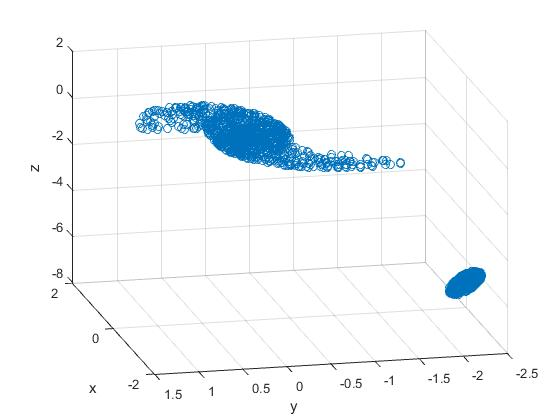
\includegraphics[scale = 0.35]{JSPAMTestPlot_xyz} & 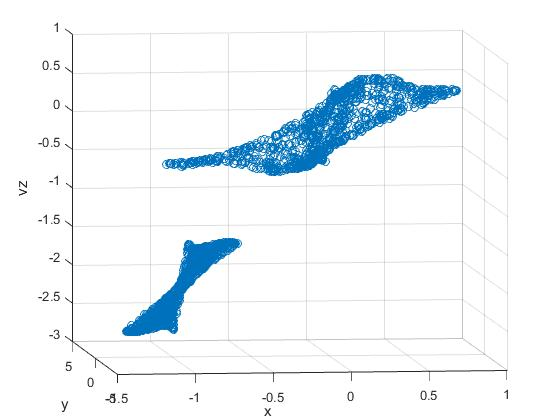
\includegraphics[scale = 0.35]{JSPAMTestPlot_xyvz}
	\end{align*}
	\caption{Final time-step of a JSPAM merger simulation (1000 particles per galaxy). Left: X-Y-Z plot. Right X-Y-Vz plot. NOTE: the graphs are viewed at two different orientations.}
\end{figure}

Given a list of \emph{final} parameters post-merger, the centers of mass are laced at theri respective positions and integrated backward in time, past the point of closest approach to a fixed starting time. Then, particle positions and velocities as well as the galactic potential are then initialized. Finally, the system is integrated forward in time, with the centers of mass back to their original positions. Since the galactic potential is a fairly complicated function which must be called many times throughout a simulation, it is assumed to be spherically symmetric, pre-calculated at a set of fixed radial distances, and stored. During simulations, the value of the potential in between these radii is calculated via linear interpolation. Since the potentials are stored, they do not change over time; however, since they originate from the centers of mass, they do translate through space. In addition to the potential, JSPAM also includes a force due to dynamical friction. This phenomenon slows objects traveling through a medium of gravitating particles by causing an increase in particle density behind the object, thus increasing the gravitational force in the retrograde direction.

\subsection{Galaxy Zoo: Mergers and Merger Wars}

From a computational perspective, the problem of finding an appropriate fitness function for comparing morphologies is a real challenge. It is difficult to find a method that is robust enough to perform on a level equivalent to that of a human. By nature, humans are excellent at pattern recognition; and where it can be difficult to ``train'' an algorithm to spot similarities between objects, humans can do it almost instinctively. For this reason, Holincheck et al. \cite{citizen} employed the help of thousands of Citizen Scientists to assist the \emph{Galaxy Zoo: Mergers} project in which they volunteered their pattern recognition abilities to determine best-fit models for 62 actual mergers.

The volunteers analyzed the morphologies of many thousands of simulations via a vote-based tournament scheme called the \emph{Merger Wars} algorithm. In a typical session, a volunteer is shown an image of the target (the actual merger) along with two simulations which model the target. The volunteer then chooses which simulation is most similar to the target, which counts as a ``win'' for one and a ``loss'' for the other. (They can also select neither image, thereby affording both images a loss.) Since it is entirely possible for images to be judged poorly, every simulation participates in multiple rounds of the tournament so that a bad round does not have a large impact on the results of the competition. The fitness of a particular simulation is then calculated as the percentage of ``wins'' it achieved, with the maximum being 1. Since an integral part of our research involved find an explicit mathematical fitness function for the merger morphologies, it was very useful to have the \emph{Merger Wars} data with which we could assess the validity of our own data.

\subsection{SDSS and MaNGA}

The end goal of our research is to construct an automated pipeline which can compare the morphologies of simulated mergers with images of actual mergers. Once we reach this stage, we will use the Sloan Digital Sky Survey's (SDSS) extensive catalog of observational data. Over the years, SDSS has provided many large, detailed data releases on collections of galactic mergers, the latest of which includes data from the Mapping Nearby Galaxies at APO (MaNGA) project. Thanks to the use of new observational tools, MaNGA has been able to capture spectra over the surface of nearly 2,000 galaxies, including many mergers. With this information, it is possible to derive the $z$-velocity fields and dispersions of the galaxies ($z$ being the axis from the telescope to the galaxy with positive $z$ in the direction of the telescope) and using these velocity fields, we will be able to apply our MCMC method for estimating the mergers' dynamical parameters.

\begin{figure}[!h]
	\centering
	\begin{align*}
		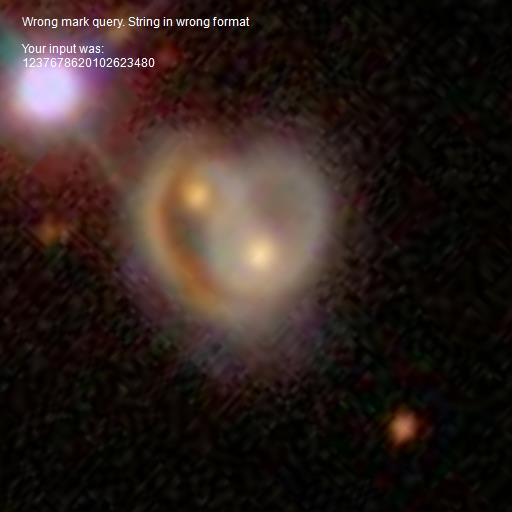
\includegraphics[scale = 0.38]{heartgalaxy} & \hspace{5mm}
		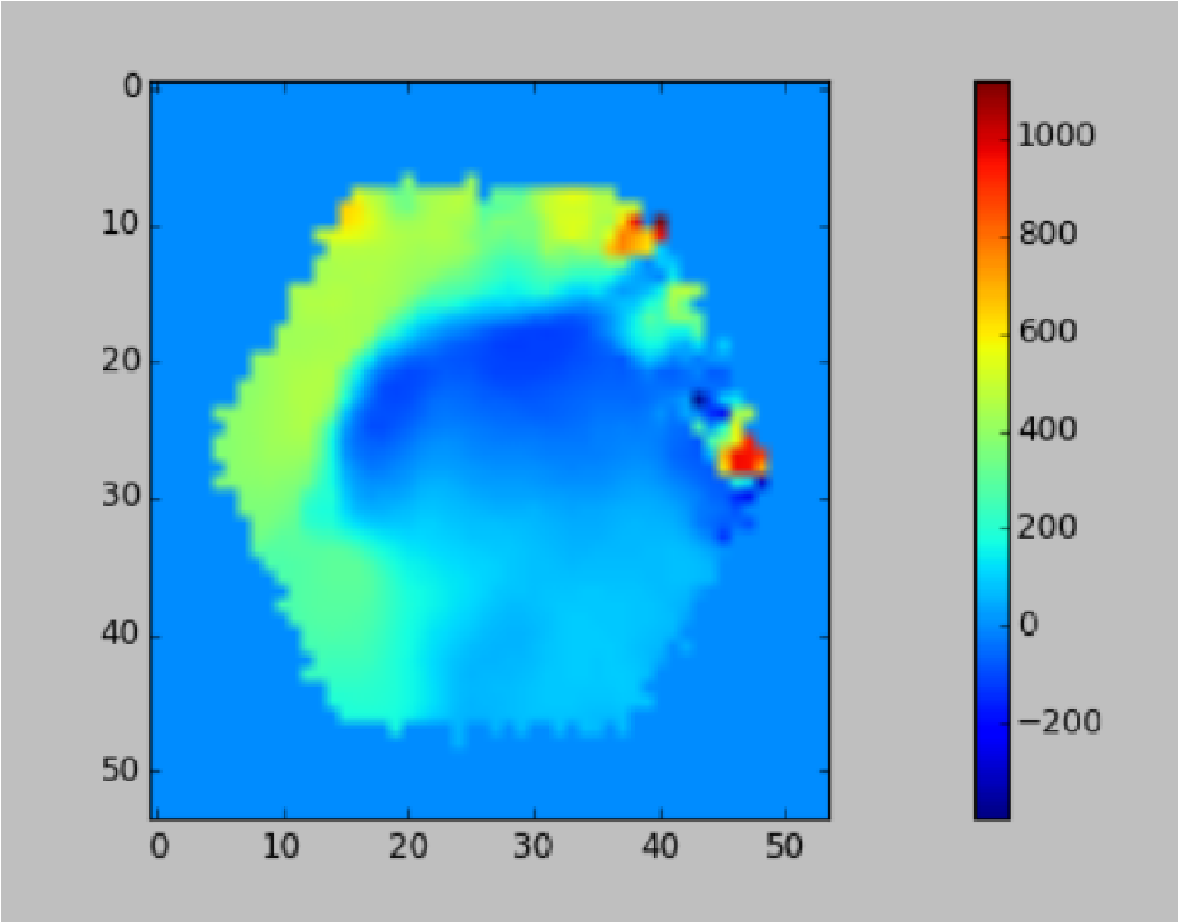
\includegraphics[scale = 0.265]{heartgalaxy_velocity}
	\end{align*}
	\caption{Visible image ($512 \times 512$ pixels) and $z$-velocity ($54 \times 54$ pixels) of a merger observed by MaNGA.}
\end{figure}

\section{Methods}

At its heart, a parameter estimation problem is essentially an optimization problem in which one minimizes a given error funciton w.r.t. a set of parameters. The two fundamental parts to the solution of such an optimization problem 1) a reliable fitness function and 2) a robust optimization algorithm. In this section, we will examine the reasoning behind the function we developed as well as the modifications we made to the canonical Metropolis-Hastings method.

\subsection{Fitness Function}

There are essentially two types of information which our fitness function may draw upon: particle positions and velocities. Obviously, however, we can't evalute our fitness function on a per-particle basis because--among many reasons--once we begin using real merger targets, we will not have per-star information for the actual mergers. (NOTE: It was very important that we kept the context of real merger targets in our minds as we experimented with the different fitness functions because whatever we decided on in the testing phase must still be able to work when applied to real targets.) Fortunately, this restriction led us to an elegant solution to the problem. The data is in the format of a $54 \times 54$ image for the $z$-velocity and a $512 \times 512$ image for visible light. Therefore, simply binning the particle number and $z$-velocity of a simulation will give us an equivalent format.

\begin{figure}[!h]
	\centering
	\begin{align*}
		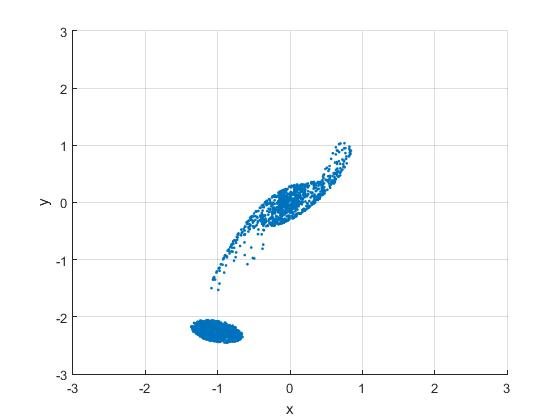
\includegraphics[scale = 0.3]{Plot_GalaxyPoints.jpg} & 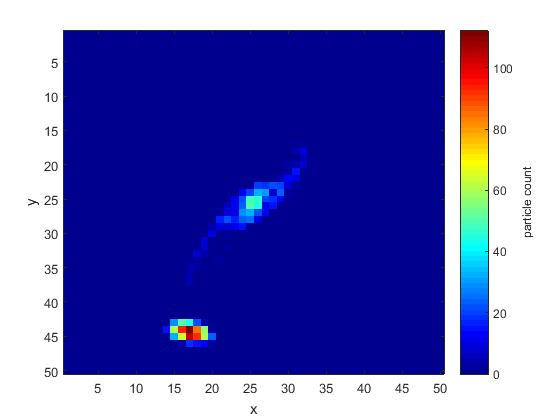
\includegraphics[scale = 0.3]{Plot_GalaxyPoints_Binned.jpg}
	\end{align*}
	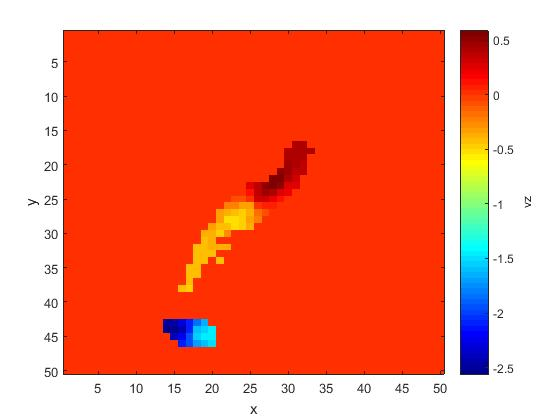
\includegraphics[scale = 0.3]{Plot_GalaxyVelocity_Binned.jpg}
		\caption{Left: a per-particle image of a merger simulation. Right: a 50x50 square-binning of the left image (high-density regions are red and low-density regions are blue). Bottom: a 50x50 square-binning of the $z$-velocities.}
\end{figure}

Binning the particle number is trivial; however, when binning the $z$-velocity, we must account for the opacity of the gas and dust within the galaxies. To do so, we bin the velocities in 3D, averageing the values of all the particles within each bin to get its value. The equation which governs the decrease in intensity of light as it passes through a medium or density $\rho$ from $z_-$ to $z_+$is:
\begin{equation}
	I(x,y,z) = I(x,y,z_-) \textrm{\hspace{2pt}exp}(-\kappa \int_{z_-}^{z_+} \rho(x,y,z) dz)
\end{equation}
Now, we use this a kernel weighting for the velocity to map it from 2D to 3D:
\begin{equation}
	v_{2D}(x,y) = \dfrac{\int_{z_-}^{z_+}v_{3D}(x,y,z)I(x,y,z)dz}{\int_{z_-}^{z_+}I(x,y,z)dz}
\end{equation}
Having binned the simulation, we have two grids representing the $x$-$y$ distribution of particle density and $z$-velocity. We now divide the fitness function into two parts, one relateing to the particle distribution and the other to the RMS error of the $z$-velocities of merger target and simulation (NOTE: Our fitness function is an error function, so small values mean high fitness):
\begin{equation}
	f(sim, tar) = (1-OvrFrac) \cdot RMS
\end{equation}
where,
\begin{equation}
	OvrFrac = \dfrac{A^{ovr}}{A^{sim}+A^{tar}-A^{ovr}}
\end{equation}
and
\begin{equation}
	RMS^2 = \sum_{k}^{} w_k(v^{sim}_k-v^{tar}_k)^2
\end{equation}
In these equations, $sim$ and $tar$ are indices referring to the \textit{simulation} and \textit{target}, respectively. $OvrFrac$--the overlap fraction--is the fraction of bins (or area, denoted by $A$) in which both the simulation and the target have particles present. RMS is the root-mean-squared error between the velocity fields only calculated over the overlapping pixels (thus, $w_k = 1$ if the pixels overlap, $w_k = 0$ otherwise). We experimented with different weighting, but none performed significantly better than this trivial case.

It is important to have both the overlap and RMS terms in the function. Consider the fact that morphologically similar mergers will have have high overlap and low velocity error, but the converse of this statement is not necessarily true. If the overlap is high, there is a proability that the velocity error could still be large, or vice versa. This probability is decreased if we include both velocity and overlap in the calculation.

\subsection{Adaptive Metropolis-Hastings}

Due to the choatic nature of the merger system, the fitness lanscape of the parameters space is incredibly complicated, having countless local maxima and minima. Consequently, any gradient-based optimization scheme would be utterly unreliable. Therefore, we chose a more robust, MCMC method: Metropolis-Hastings. Given an initial guess, this method takes random jumps through parameter space in an attempt to find the parameters set which most likely produced the given data. To maximize this probability, we calculate the log-probability at each step,
\begin{equation}
	log(P) = -n_{bin}^2 \cdot (\dfrac{1}{2}log(2 \pi \sigma^2) + \dfrac{f(sim,tar)^2}{2 \sigma^2})
\end{equation}
where the images are $n_{bin} \times n_{bin}$ and $\sigma$ is a value between 0.0-0.5.



How in depth do I go about Metropolis?


\section{Testing, Results, and Analysis}
During testing all of our binning resolution ranged between $30\times30$ to $50\times50$ and particle numbers were between $5000$ and $30000$ per galaxy. Our method of testing consisted of running many instances of the method in parallel all with the same target and initial parameters, but allowing different paths through parameter space. We would then plot the Markov chains to see how many--if any--instances eventually reached below a given error threshold. Once we found what appeared to be a successful instance, we would plot several mergers along the Markov chain to see how much improvement was made.

When testing our method, we were very impressed by its ability to determine morphological matches to the target. 







\section{Conclusions}





\section*{Acknowledgments}
We would like to acknowledge the assistance of volunteers in putting
together this example manuscript and supplement.

\bibliographystyle{siamplain}
\bibliography{references}



\begin{thebibliography}{10}

\bibitem{citizen} A. Holincheck, J. Wallin, K. Borne, L. Fortson, C. Lintott, A M. Smith, S. Bamford, W. Keel, and M. Parrish, ``Galaxy Zoo: Mergers - Dynamical Models of Interacting Galaxies.'' \textit{MNRAS}, (2016). Vol. 459, Is. 1, 720-745.

\bibitem{galaxyFE} H. Mo, F. Bosch, and S. White, \textit{Galaxy Formation and Evolution}, 2010, Cambridge University Press.

\bibitem{jspam} J. Wallin, A. Holincheck, and A. Harvey, ``JSPAM: A restricted three-body code for simulating interacting galaxies.'' \textit{Astronomy and Computing} 16, (2016). 26-33.


\end{thebibliography}


\end{document}




